% A LaTeX template for MSc Thesis submissions to 
% Politecnico di Milano (PoliMi) - School of Industrial and Information Engineering
%
% S. Bonetti, A. Gruttadauria, G. Mescolini, A. Zingaro
% e-mail: template-tesi-ingind@polimi.it
%
% Last Revision: October 2021
%
% Copyright 2021 Politecnico di Milano, Italy. NC-BY

\documentclass{config/polimi_template}

%------------------------------------------------------------------------------
%	REQUIRED PACKAGES AND  CONFIGURATIONS
%------------------------------------------------------------------------------

% CONFIGURATIONS
%Importante!!!
\usepackage{epstopdf}

\usepackage{comment}
\usepackage{parskip} % For paragraph layout
\usepackage{setspace} % For using single or double spacing
\usepackage{emptypage} % To insert empty pages
\usepackage{multicol} % To write in multiple columns (executive summary)
\setlength\columnsep{15pt} % Column separation in executive summary
\setlength\parindent{0pt} % Indentation
\raggedbottom

% PACKAGES FOR TITLES
\usepackage{titlesec}
% \titlespacing{\section}{left spacing}{before spacing}{after spacing}
\titlespacing{\section}{0pt}{3.3ex}{2ex}
\titlespacing{\subsection}{0pt}{3.3ex}{1.65ex}
\titlespacing{\subsubsection}{0pt}{3.3ex}{1ex}
\usepackage{color}

% PACKAGES FOR LANGUAGE AND FONT
\usepackage[english]{babel} % The document is in English  
\usepackage[utf8]{inputenc} % UTF8 encoding
\usepackage[T1]{fontenc} % Font encoding
\usepackage[11pt]{moresize} % Big fonts

% PACKAGES FOR IMAGES
\usepackage{graphicx}
\usepackage{transparent} % Enables transparent images
\usepackage{eso-pic} % For the background picture on the title page
\usepackage{subfig} % Numbered and caption subfigures using \subfloat.
\usepackage{tikz} % A package for high-quality hand-made figures.
\usetikzlibrary{}
\graphicspath{{./Images/}} % Directory of the images
\usepackage{amsthm} % Coloured "Theorem"
\usepackage{thmtools}
\usepackage{xcolor}
\usepackage{float}

% STANDARD MATH PACKAGES
\usepackage{amsmath}
\usepackage{amssymb}
\usepackage{amsfonts}
\usepackage{bm}
\usepackage[overload]{empheq} % For braced-style systems of equations.
\usepackage{fix-cm} % To override original LaTeX restrictions on sizes

% PACKAGES FOR TABLES
\usepackage{tabularx}
\usepackage{longtable} % Tables that can span several pages
\usepackage{colortbl}

% PACKAGES FOR ALGORITHMS (PSEUDO-CODE)
\usepackage{algorithm}
\usepackage{algorithmic}

% PACKAGES FOR REFERENCES & BIBLIOGRAPHY
\usepackage[
    colorlinks=true,
    linkcolor=black,
    anchorcolor=black,
    citecolor=black,
    filecolor=black,
    menucolor=black,
    runcolor=black,
    urlcolor=black
]{hyperref} % Adds clickable links at references
\usepackage{cleveref}
\usepackage[square, numbers, sort&compress]{natbib} % Square brackets, citing references with numbers, citations sorted by appearance in the text and compressed
\bibliographystyle{abbrvnat} % You may use a different style adapted to your field

% OTHER PACKAGES
\usepackage{pdfpages} % To include a pdf file
\usepackage{afterpage}
\usepackage{lipsum} % DUMMY PACKAGE
\usepackage{fancyhdr}
\usepackage{wasysym} % For the headers
\usepackage{rotating}
\usepackage{listings}
%%
% Alloy language definition for using with the listings package.
%
% 2017, Daniel Andrade
% BSD 3-Clause License
%%
\lstdefinelanguage{alloy}{
    morekeywords={
        module, open, as,
        private, abstract, sig, extends, in,
        lone, some, one, disj,
        fact, pred, fun, assert,
        run, check,
        for, but, exactly,
        this, not, implies, else, let,
        not, no, set, all, sum,
        iff, or, Int, and,
        none, univ, iden
    },
    sensitive=true,
    morecomment=[l]{//},
    morecomment=[l]{--},
    morecomment=[s]{/*}{*/},
    morestring=[b]{"},
%literate={->}{$\rightarrow$}1
% replacing characters can cause problems when copying from PDF to editor
}[keywords,comments,strings]
\fancyhf{}

% Input of configuration file. Do not change conf.tex file unless you really know what you are doing. 
% Define blue color typical of polimi
\definecolor{bluepoli}{cmyk}{0.4,0.1,0,0.4}

% Custom theorem environments
\declaretheoremstyle[
    headfont=\color{bluepoli}\normalfont\bfseries,
    bodyfont=\color{black}\normalfont\itshape,
]{colored}

% Set-up caption colors
\captionsetup[figure]{labelfont={color=bluepoli}} % Set colour of the captions
\captionsetup[table]{labelfont={color=bluepoli}} % Set colour of the captions
\captionsetup[algorithm]{labelfont={color=bluepoli}} % Set colour of the captions

\theoremstyle{colored}
\newtheorem{theorem}{Theorem}[chapter]
\newtheorem{proposition}{Proposition}[chapter]

% Enhances the features of the standard "table" and "tabular" environments.
\newcommand\T{\rule{0pt}{2.6ex}}
\newcommand\B{\rule[-1.2ex]{0pt}{0pt}}

% Pseudo-code algorithm descriptions.
\newcounter{algsubstate}
\renewcommand{\thealgsubstate}{\alph{algsubstate}}
\newenvironment{algsubstates}
{\setcounter{algsubstate}{0}%
\renewcommand{\STATE}{%
    \stepcounter{algsubstate}%
    \Statex {\small\thealgsubstate:}\space}}
{}

% New font size
\newcommand\numfontsize{\@setfontsize\Huge{200}{60}}

% Title format: chapter
\titleformat{\chapter}[hang]{
    \fontsize{50}{20}\selectfont\bfseries\filright}{\textcolor{bluepoli} \thechapter\hsp\hspace{2mm}\textcolor{bluepoli}{|   }\hsp}{0pt}{\huge\bfseries \textcolor{bluepoli}
}

% Title format: section
\titleformat{\section}
{\color{bluepoli}\normalfont\Large\bfseries}
{\color{bluepoli}\thesection.}{1em}{}

% Title format: subsection
\titleformat{\subsection}
{\color{bluepoli}\normalfont\large\bfseries}
{\color{bluepoli}\thesubsection.}{1em}{}

% Title format: subsubsection
\titleformat{\subsubsection}
{\color{bluepoli}\normalfont\large\bfseries}
{\color{bluepoli}\thesubsubsection.}{1em}{}

% Shortening for setting no horizontal-spacing
\newcommand{\hsp}{\hspace{0pt}}

\makeatletter
% Renewcommand: cleardoublepage including the background pic
\renewcommand*\cleardoublepage{%
    \clearpage\if@twoside\ifodd\c@page\else
    \null
    \AddToShipoutPicture*{\BackgroundPic}
    \thispagestyle{empty}%
    \newpage
    \if@twocolumn\hbox{}\newpage\fi\fi\fi}
\makeatother

%For correctly numbering algorithms
\numberwithin{algorithm}{chapter}

%----------------------------------------------------------------------------
%	NEW COMMANDS DEFINED
%----------------------------------------------------------------------------

%----------------------------------------------------------------------------
%	ADD YOUR PACKAGES (be careful of package interaction)
%----------------------------------------------------------------------------

%----------------------------------------------------------------------------
%	ADD YOUR DEFINITIONS AND COMMANDS (be careful of existing commands)
%----------------------------------------------------------------------------

\definecolor{dkgreen}{rgb}{0,0.6,0}
\definecolor{gray}{rgb}{0.5,0.5,0.5}
\definecolor{mauve}{rgb}{0.58,0,0.82}

\lstset{frame=tb,
    language=alloy,
    aboveskip=3mm,
    belowskip=3mm,
    showstringspaces=false,
    columns=flexible,
    basicstyle={\small\ttfamily},
    numbers=none,
    numberstyle=\tiny\color{gray},
    keywordstyle=\bf\color{blue},
    commentstyle=\it\color{dkgreen},
    stringstyle=\color{mauve},
    breaklines=true,
    breakatwhitespace=true,
    tabsize=3
}

%----------------------------------------------------------------------------
%	BEGIN OF YOUR DOCUMENT
%----------------------------------------------------------------------------

\begin{document}
    \fancypagestyle{plain}{%
        \fancyhf{} % Clear all header and footer fields
        \fancyhead[RO,RE]{\thepage} %RO=right odd, RE=right even
        \renewcommand{\headrulewidth}{0pt}
        \renewcommand{\footrulewidth}{0pt}}

%----------------------------------------------------------------------------
%	TITLE PAGE
%----------------------------------------------------------------------------

    \pagestyle{empty} % No page numbers
    \frontmatter % Use roman page numbering style (i, ii, iii, iv...) for the preamble pages

    \puttitle{
        title=Software Engineering 2\\Requirements Analysis and\\Specification Document,
        name1=Federico Zanca - XXXXXXXX, % Author Name and Surname
        name2=Federico Costantini - XXXXXXXX,
        name3=Michele Zhenghao Zhuge - XXXXXXXX,
        academicyear=2023-2024,
    } % These info will be put into your Title page

%----------------------------------------------------------------------------
%	PREAMBLE PAGES: ABSTRACT (inglese e italiano), EXECUTIVE SUMMARY
%----------------------------------------------------------------------------
    \startpreamble
    \setcounter{page}{1} % Set page counter to 1

%----------------------------------------------------------------------------
%	LIST OF CONTENTS/FIGURES/TABLES/SYMBOLS
%----------------------------------------------------------------------------

% TABLE OF CONTENTS
    \thispagestyle{empty}
    \tableofcontents % Table of contents
    \thispagestyle{empty}
    \cleardoublepage

%-------------------------------------------------------------------------
%	THESIS MAIN TEXT
%-------------------------------------------------------------------------

    \addtocontents{toc}{\vspace{2em}} % Add a gap in the Contents, for aesthetics
    \mainmatter % Begin numeric (1,2,3...) page numbering


    \chapter{Introduction}
    \label{ch:introduction}%
    CodeKataBattle (CKB) emerges as a pivotal platform in the evolving landscape of software development education. 
As the paradigm shifts towards enhancing coding proficiency, CKB provides a dynamic arena where students engage in collaborative code kata battles, 
refining their skills through hands-on challenges. 

Educators orchestrate these battles within tournaments, defining parameters such as group sizes, deadlines, and scoring configurations. 
Facilitating a test-first approach, CKB seamlessly integrates with GitHub, automating workflows and enabling real-time evaluations. 
As scores evolve, students and educators gain insights into individual and team performances, fostering a competitive yet collaborative learning environment. 

Beyond individual battles, CKB aggregates personal tournament scores, offering a comprehensive view of students' progress. 
Introducing gamification with badges, educators recognize achievements, enhancing the overall learning experience. 
In essence, CodeKataBattle propels software development education into a new era, blending competition, collaboration, and skill refinement within a cutting-edge platform.
\newpage


\section{Purpose}
\label{sec:purpose}%

\subsection{Goals}
\label{subsec:goals}%
\newcounter{g}
\setcounter{g}{1}
\newcommand{\cg}{\theg\stepcounter{g}}
\verb|CodeKataBattle(CKB)| platform serves as a dynamic and interactive space for students and educators, 
promoting continuous learning, healthy competition, and recognition of individual and team accomplishments in the realm of software development.

Students can engage in coding challenges by joining battles individually or forming teams within specified limits.
By actively contributing to code repositories on GitHub, following a test-first approach, they strive to achieve high scores in battles, contributing to their personal tournament ranking.
Eventually work towards earning gamification badges based on their performance and achievements in tournaments.

Educators instead, develop and publish code kata battles, setting criteria for evaluation and deadlines.
They will assess student submissions, providing manual scores if required and shaping the final rankings, also defining gamification badges with specific rules and criteria to recognize outstanding achievements.
Further more they will oversee the progression of tournaments, including opening, closing, and notifying participants.

Below there's a table that lists all the goals of the \verb|CKB| platform:
\begin{center}
    \begin{longtable}{ |l|p{0.9\linewidth}| }
        \hline
        \textbf{ID} & \textbf{Description}                                                                   \\
        \hline
        G\cg        & The platform should allow educators to set up code kata battles with configurable parameters.\\
        \hline
        G\cg        & The platform should allow third party platforms integration.\\
        \hline
        G\cg        & The platform should allow students to join battles individually or form teams within specified size limits.\\
        \hline
        G\cg        & The platform should allow users to see real time updates on current tournaments and battles\\
        \hline
        G\cg        & The platform should have automated evaluations of code submissions.\\
        \hline
        G\cg        & The platform should allow educators to manually evaluate and assign scores for optional factors at the end of each battle.                     \\
        \hline
        G\cg        & The platform should allow users to visualize informations about another user.\\
        \hline
        G\cg        & The platform should be able to notify users about current events\\
        \hline
        G\cg        & The platform should allow educators to create new gamification badges.\\
        \hline
        \caption{The goals.}
        \label{tab:goals_tab}%
    \end{longtable}
\end{center}

%\newpage


\section{Scope}
\label{sec:scope}%
The scope of the requirements analysis and specification document - RASD - is to provide a detailed description of the requirements for the project.
It outlines what the system or product should do and how it should behave, as well as any constraints or limitations on its design and implementation.
The RASD is based on a thorough analysis of the needs and requirements of the stakeholders.
The scope of the RASD will cover all of the essential aspects of the system and provide a clear and detailed roadmap for its development.

\subsection{World phenomena}
\label{subsec:world_phenomena}%
\newcounter{wp}
\setcounter{wp}{1}
\newcommand{\cwp}{\thewp\stepcounter{wp}}
\begin{center}
    \begin{longtable}{ |l|p{0.8\linewidth}| }
        \hline
        \textbf{ID} & \textbf{Description}                                                \\
        \hline
        WP\cwp      & Educators create new tournaments for coding challenges.                          \\
        \hline
        WP\cwp      & Students seek opportunities to improve their software development skills.   \\
        \hline
        WP\cwp      & Educators define code kata battles with project details and evaluation criteria. \\
        \hline
        WP\cwp      & Students aim to participate in code kata battles individually or form teams.          \\
        \hline
        WP\cwp      & Students are informed of upcoming battles when subscribed to a tournament.                \\
        \hline
        WP\cwp      & Students form teams within specified limits for a code kata battle.                 \\
        \hline
        WP\cwp      & Students aim to visualize their personal tournament scores and earned badges.         \\
        \hline
        WP\cwp      & Educators define gamification badges and rules when creating a tournament.      \\
        \hline
        WP\cwp      & At the end of each battle, the CKB platform notifies students of the final battle rank and updates personal tournament scores.                       \\
        \hline
        WP\cwp      & Educators can close tournaments, and the platform notifies all students when the final tournament rank becomes available. \\
        \hline
        WP\cwp      & Students and educators seek information about ongoing tournaments, ranks, and profiles with badges.                      \\
        \hline
        \caption{World Phenomenas.}
        \label{tab:worldph_tab}%
    \end{longtable}
\end{center}

\subsection{Shared phenomena}
\label{subsec:shared_phenomena}%
\newcounter{sp}
\setcounter{sp}{1}
\newcommand{\csp} {\thesp\stepcounter{sp}}
\begin{center}
    \begin{longtable}{ |l|p{0.5\linewidth}|l|l| }
        \hline
        \textbf{ID} & \textbf{Description}                                                                                                          & \textbf{Controller} & \textbf{Observer} \\
        \hline
        SP\csp      & Student subscribes to the CKB platform for notifications.\                                                                    & Student                 & CKB Platform             \\
        \hline
        SP\csp      & Educator creates a new tournament, specifying details and criteria.\                                                          & Educator                 & CKB Platform            \\
        \hline
        SP\csp      & CKB Platform notifies subscribed students about a new tournament.\                                                            & CKB Platform                & Student             \\
        \hline
        SP\csp      & Student forms a team within specified limits for a code kata battle.\                                                         & Student               & CKB Platform               \\
        \hline
        SP\csp      & Educator sets up a code kata battle, including project details and evaluation criteria.\                                      & Educator                 & CKB Platform            \\
        \hline
        SP\csp      & CKB Platform generates a GitHub repository for a code kata battle.                                                            & CKB Platform               & Student               \\
        \hline
        SP\csp      & Student forks the GitHub repository and sets up automated workflows.                                                          & Student                 & CKB Platform             \\
        \hline
        SP\csp      & Student pushes commits to GitHub, triggering automated evaluation.                                                            & Student              & CKB Platform               \\
        \hline
        SP\csp      & Automated evaluation includes functional correctness, timeliness, and code quality.                                           & CKB Platform               & Student               \\
        \hline
        SP\csp      & Educator manually evaluates optional factors, such as personal scores.                                                        & Educator               & CKB Platform              \\
        \hline
        SP\csp      & CKB Platform updates battle scores in real-time based on new commits.                                                         & CKB Platform              & Student               \\
        \hline
        SP\csp      & Students and educators observe the evolving rank during a battle.                                                             & Student               & CKB Platform             \\
        \hline
        SP\csp      & CKB Platform notifies students when the final battle rank is available.                                                       & CKB Platform              & Student               \\
        \hline
        SP\csp      & CKB Platform updates personal tournament scores at the end of a battle.                                                       & CKB Platform               & Student              \\
        \hline
        SP\csp      & Educator closes a tournament, and the platform notifies students of the final rank.                                           & Educator                & CKB Platform            \\
        \hline
        SP\csp      & Educator defines gamification badges and rules when creating a tournament.                                                    & Educator              & CKB Platform              \\
        \hline
        SP\csp      & Students earn gamification badges based on their performance and achievements.                                                & Student                 & CKB Platform            \\
        \hline
        SP\csp      & Students and educators visualize ongoing tournaments, ranks, and profiles with badges.                                        & Student               & CKB Platform             \\
        \hline
        
        \caption{Shared Phenomenas.}
        \label{tab:sharedph_tab}%
    \end{longtable}
\end{center}


\section{Definition, Acronyms, Abbreviations}
\label{sec:definition_acronyms_abbreviations}%
\begin{table}[H]
    \begin{center}
        \begin{tabular}{ |l|l| }
            \hline
            \textbf{Acronyms} & \textbf{Definition}                              \\
            \hline
            CKB              & Code Kata Battle                      \\
            \hline
            RASD              & Requirements Analysis and Specification Document \\
            \hline
        \end{tabular}
        \caption{Acronyms used in the document.}
        \label{tab:acronyms}%
    \end{center}
\end{table}


\section{Revision history}
\label{sec:revision_history}%
This version of RASD differs from the previous one for:
\begin{itemize}
    \item In section 1.2, we have inserted a brief description about the scope of the document.
    \item In section 3.1.3, we have added the Navigator System software interface.
    \item In section 3.2.1, we have added the requirements R70 to the table and updated the requirement R39.
    \item In section 3.4, we have updated some sequence diagrams to make them coherent with the ones presented in the DD\@.
\end{itemize}


\section{Reference Documents}
\label{sec:reference_documents}%
%%\begin{itemize}
%%\end{itemize}


\section{Document Structure}
\label{sec:document_structure}%
The document is structured in six sections, as described below.

First section introduce the goals of the project, purposes, and a brief analysis on world and shared phenomena;
abbreviations and definitions useful to understand the problem are listed as well.

The following section, the second one, provides an overall description of the problem: here further
details on domain and scenarios are included, aside from more product and user characteristics, assumptions,
dependencies and constraints.

Later on, the third section focuses on the specific requirements and provides a more detailed analysis of external
interface requirements, functional requirements and performance requirements.

Lastly, the fourth section provides a formal analysis, using alloy.
This chapter is crucial to prove the correctness of the model described in the previous sections, and should focus on
reporting results of the checks performed and meaningful assertions.

Section five reports the effort spent by each group member in the redaction of this document, meanwhile the last
section simply lists bibliography references and other resources used to redact this document.



    \chapter{Overall Description}
    \label{ch:overall_description}%
    Hey


    \chapter{Specific Requirements}
    \label{ch:specific_requirements}%
    \section{External Interface Requirements}
\label{sec:external_interface_requirements}%

\subsection{User Interfaces}
\label{subsec:user_interfaces}%
The \verb|CodeKataBattle (CKB)| platform is accessed via an intuitive and responsive web interface compatible with major browsers (Chrome, Firefox, Safari, etc.).
Educators enjoy a dedicated dashboard for effortless creation and management of tournaments, battles, and badges. This dashboard provides a comprehensive view of ongoing battles, tournament scores, and badge achievements.
Students utilize a user-friendly dashboard for team formation, battle participation, and progress tracking. It streamlines team formation, displays upcoming battles, current ranks, and summarizes earned badges.
GitHub seamlessly integrates into the platform for code versioning and automated testing. Students can easily fork repositories, set up GitHub Actions, and monitor build and test results within the \verb|CKB| platform.
To keep all stakeholders informed, the platform employs a robust notification system. This system supports both email notifications and in-platform alerts, 
ensuring timely updates for educators and students on critical events like upcoming deadlines or changes in battle status.

\subsection{Hardware Interfaces}
\label{subsec:hardware_interfaces}%
The \verb|CKB| platform prioritizes accessibility by ensuring compatibility across a diverse range of devices. 
Users can seamlessly access the platform from desktop computers, laptops, tablets, and smartphones. This inclusivity caters to the varied preferences and device usage patterns of our user base. 
The platform's responsive design ensures that the user interface adapts fluidly to different screen sizes, providing an optimal experience regardless of the device used. 
This commitment to device compatibility aims to enhance user convenience and flexibility, promoting a versatile and user-centric engagement with the \verb|CKB| platform.

\subsection{Software Interfaces}
\label{subsec:software_interfaces}%
The \verb|CKB| platform seamlessly communicates with GitHub via APIs, enabling functionalities such as repository creation, commit tracking, and automated test processes.
To ensure a secure integration, the platform should smoothly connect with GitHub APIs, facilitating automated workflows triggered by student commits.
Additionally, the platform harnesses static analysis tools to assess code quality comprehensively.
Incorporating these tools seamlessly, educators can tailor automated evaluations by configuring specific aspects like security, reliability, and maintainability. This flexibility ensures a nuanced understanding of the code's overall quality.

\subsection{Communication Interfaces}
\label{subsec:communication_interfaces}%
The platform actively engages in communication with students, delivering notifications, battle updates, and final results in a secure manner through HTTPS. A reliable messaging system ensures timely information dissemination to students.
Similarly, educators stay well-informed through the platform, receiving notifications and updates on battle progress and final results. Secure communication channels, similar to those used for students, guarantee the confidentiality and reliability of information relayed to educators.
For the configuration of badges and rules, educators seamlessly use the platform to define new badges, rules, and associated variables. Ensuring a user-friendly interface, educators can make real-time adjustments, with changes promptly reflecting across the platform. This intuitive process empowers educators to tailor the platform to their evolving requirements effortlessly.

\section{Functional Requirements}
\label{sec:functional_requirements}%

\subsection{Requirements}
\label{subsec: requirements}%
The \verb|CKB| platform offers several functionalities to both educators and students.
In the following table they are listed all the detected requirements that the platform should respect in order to guarantee
the satisfiability of the goals:
\newpage
\newcounter{req}
\setcounter{req}{1}
\newcommand{\creq}{\thereq\stepcounter{req}}
\textbf{Educators}
\begin{center}
    \begin{longtable}{|l|p{0.9\linewidth}|}
        \hline
        \textbf{ID} & \textbf{Description}                                                                                                                             \\
        \hline
        R\creq      & The \verb|CKB| platform shall allow educators to create an account.                                                                    \\
        \hline
        R\creq      & The \verb|CKB| platform shall allow educators to log in.                                                                                 \\
        \hline
        R\creq      & The \verb|CKB| platform shall allow educators to create a new tournament.                                                                \\
        \hline
        R\creq      & The \verb|CKB| platform shall allow educators to set the minimum and maximum number of students per group for a tournament.                                                        \\
        \hline
        R\creq      & The \verb|CKB| platform shall allow educators to upload a code kata battle.                                                                         \\
        \hline
        R\creq      & The \verb|CKB| platform shall allow educators to grant permissions to other educators to create battles within a specific tournament.                                                      \\
        \hline
        R\creq      & The \verb|CKB| platform shall enable educators to include a battle to a specific tournament.                                                      \\
        \hline
        R\creq      & The \verb|CKB| platform shall allow educators to include a description for a battle.                                                                \\
        \hline
        R\creq      & The \verb|CKB| platform shall allow educators to include a software project with test cases.                                                                \\
        \hline
        R\creq      & The \verb|CKB| platform shall allow educators to set a registration deadline for a battle within a tournament.                                          \\
        \hline
        R\creq      & The \verb|CKB| platform shall allow educators to set a final submission deadline for a battle within a tournament.                                                                  \\
        \hline
        R\creq      & The \verb|CKB| platform shall allow educators to set additional configurations for scoring, including functional aspects and quality level criteria.                               \\
        \hline
        R\creq      & The \verb|CKB| platform shall allow educators to close a tournament.                                                  \\
        \hline
        R\creq      & The \verb|CKB| platform shall allow an educator to define optional manual evaluation criteria for score assignment in battles.   \\
        \hline
        R\creq      & The \verb|CKB| platform shall allow educators to manually evaluate and assign scores to teams.                                           \\
        \hline
        R\creq      & The \verb|CKB| platform shall allow educators and students to visualize the gamification badges.                                                      \\
        \hline
        R\creq      & The \verb|CKB| platform shall allow educators to define new badges for gamification.                                                             \\
        \hline
        R\creq      & The \verb|CKB| platform shall allow educators to define new rules associated with the badges.                                                      \\
        \hline
        R\creq      & The \verb|CKB| platform shall allow educators to define new variables associated with the badges.                                                      \\
        \hline
        R\creq      & The \verb|CKB| platform shall allow all students and educators to see the ranking of each ongoing tournament with the score of each student subscribed.\\
        \hline
        \caption{Educator Requirements.}
        \label{tab: req}%
    \end{longtable}
\end{center}

\textbf{Students}
\begin{center}
    \begin{longtable}{|l|p{0.9\linewidth}|}
        \hline
        \textbf{ID} & \textbf{Description}                                                                                                                             \\
        \hline
        R\creq      & The \verb|CKB| platform shall not allow students to participate a tournament after the registration deadline.                                                      \\
        \hline
        R\creq      & The \verb|CKB| platform shall not allow students to participate a battle after the registration deadline.                                                      \\
        \hline
        R\creq      & The \verb|CKB| platform shall allow students to subscribe to a tournament within a specified deadline.                                                  \\
        \hline
        R\creq      & The \verb|CKB| platform shall allow students to create teams for a specific battle within a tournament.                                                      \\
        \hline
        R\creq      & The \verb|CKB| platform shall allow students to join teams for a specific battle within a tournament.                                                      \\
        \hline
        R\creq      & The \verb|CKB| platform shall allow students to invite other participants to the same group.                               \\
        \hline
        R\creq      & The \verb|CKB| platform shall allow students to accept an invitation.                               \\
        \hline
        R\creq      & The \verb|CKB| platform shall allow students to reject an invitation.                               \\
        \hline
        R\creq      & The \verb|CKB| platform shall allow students to join a battle without a team.                               \\
        \hline
        R\creq      & The \verb|CKB| platform shall allow students to upload a solution for a specific battle on behalf of the team.                                                      \\
        \hline
        \caption{Student Requirements.}
        \label{tab: req}%
    \end{longtable}
\end{center}

\textbf{Platform}
\begin{center}
    \begin{longtable}{|l|p{0.9\linewidth}|}
        \hline
        \textbf{ID} & \textbf{Description}                                                                                                                             \\
        \hline
        R\creq      & The \verb|CKB| platform shall notify all subscribed students of a new battle and its details within a specific tournament.                               \\
        \hline
        R\creq      & The \verb|CKB| platform shall notify all subscribed students of a new tournament and its details.                               \\
        \hline
        R\creq      & The \verb|CKB| platform shall create a GitHub repository for each battle.                                        \\
        \hline
        R\creq      & send a link to the Github repository associated to a battle to all members of subscribed teams upon expiration of the registration deadline. \\
        \hline
        R\creq      & The \verb|CKB| platform shall be able to be informed of new students' commits by Github Actions workflows. \\
        \hline
        R\creq      & The \verb|CKB| platform shall be able to pull the latest sources from the forks of the Github repository provided. \\
        \hline
        R\creq      & The \verb|CKB| platform shall be able to run the testcases on the code uploaded by students and determine if the code is a valid solution for the exercise.\\
        \hline
        R\creq      & The \verb|CKB| platform shall inform students of the mandatory automated evaluation criteria, including functional aspects, timeliness, and source code quality.                                        \\
        \hline
        R\creq      & The \verb|CKB| platform shall automatically update the battle score of a team based on GitHub commits and test results.                                   \\
        \hline
        R\creq      & The \verb|CKB| platform shall automatically close a finished battle.                                                      \\
        \hline
        R\creq      & The \verb|CKB| platform shall assign or update battle scores to each team of the battle.                                                      \\
        \hline
        R\creq      & The \verb|CKB| platform shall calculate and update the personal tournament score of each student based on their performance in battles.                    \\
        \hline
        R\creq      & The \verb|CKB| platform shall be able to create a ranking of teams for every tournament.                                                      \\
        \hline
        R\creq      & The \verb|CKB| platform shall keep track of time elapsed from the start of a CKB and the final submissions of each team. \\
        \hline
        R\creq      & The \verb|CKB| platform shall be able to use static analysis tools to evaluate the quality of the code submitted by teams in terms of security, reliability, maintainability and other aspects defined by the educator who created the battle. \\
        \hline
        R\creq      & The \verb|CKB| platform shall notify all students involved in a tournament when it is closed and the final ranking is available.                                                       \\
        \hline
        R\creq      & The \verb|CKB| platform shall visualize ongoing tournaments and their ranks for all users.                                                                 \\
        \hline
        R\creq      & The \verb|CKB| platform shall display collected badges on the profile of both students and educators.                                                                    \\
        \hline
        \caption{Platform Requirements.}
        \label{tab: req}%
    \end{longtable}
\end{center}

\subsection{Mapping on goals}
\label{subsec: map_on_g}%
In the following section it is shown how the relation $R\land D \models G$ holds.
In particular, at first it is shown a traceability matrix that associates domain assumptions and requirements to each goal.
After that, to facilitate reading, the section reports the text of all the assumptions and all the requirements related to each goal.
\newcounter{mg}
\setcounter{mg}{1}
\newcommand{\cmg}{\themg\stepcounter{mg}}
\begin{center}
    \begin{longtable}{|p{0.06\linewidth}|p{0.34\linewidth}|p{0.6\linewidth}|}
        \hline
        \textbf{Goal} & \textbf{Domain assumptions}                       & \textbf{Requirements}                                                               \\
        \hline
        G\cmg         &                             & R23, R24, R25, R29, R30                        \\
        \hline
        G\cmg         &                             & R24, R25, R26, R27, R28                                      \\
        \hline
        G\cmg         &                             & R1, R2, R3, R4, R5, R6, R7, R8, R9, R10, R11, R12, R13, R14, R15, R16, R17, R18, R19, R20                                \\
        \hline
        G\cmg         &                             & R33, R34, R35, R36, R37, R38, R39              \\
        \hline
        G\cmg         &                             & R20, R29, R30, R44                               \\
        \hline
        G\cmg         &                             & R41, R42, R45                     \\
        \hline
        G\cmg         &                             & R46, R47                                \\
        \hline
        G\cmg         &                             & R48                                                   \\
        \hline
        G\cmg         &                             & R16, R17, R18, R19, R48                                               \\
        \hline
        \caption{Mapping on goals.}
        \label{tab: map_on_g}%
    \end{longtable}
\end{center}

In this section, it will be shown the functional requirements and the domain assumption related to each goal.
\begin{itemize}

    \item \textbf{{[G.1]} Enable students to enhance their software development skills through coding challenges.}
    \begin{itemize}
        \item \textbf{[R.23]} The \verb|CKB| platform shall allow students to subscribe to a tournament within a specified deadline.
        \item \textbf{[R.24]} The \verb|CKB| platform shall allow students to create teams for a specific battle within a tournament.
        \item \textbf{[R.25]} The \verb|CKB| platform shall allow students to join teams for a specific battle within a tournament. 
        \item \textbf{[R.29]} The \verb|CKB| platform shall allow students to join a battle without a team. 
        \item \textbf{[R.30]} The \verb|CKB| platform shall allow students to upload a solution for a specific battle on behalf of the team.
        \item \textbf{[D.1]}
    \end{itemize}

    \item \textbf{{[G.2]} Facilitate peer learning and collaboration by allowing students to form teams and work together on coding exercises. }
        \begin{itemize}
            \item \textbf{[R.24]} The \verb|CKB| platform shall allow students to create teams for a specific battle within a tournament.
            \item \textbf{[R.25]} The \verb|CKB| platform shall allow students to join teams for a specific battle within a tournament.
            \item \textbf{[R.26]} The \verb|CKB| platform shall allow students to invite other participants to the same group. 
            \item \textbf{[R.27]} The \verb|CKB| platform shall allow students to join a battle without a team.
            \item \textbf{[R.28]} The \verb|CKB| platform shall allow students to reject an invitation.
            \item \textbf{[D.1]}
        \end{itemize}

        \item \textbf{{[G.3]} Provide educators with a platform to create and manage coding challenges tailored to specific learning objectives. }
        \begin{itemize}
            \item \textbf{[R.1]} The \verb|CKB| platform shall allow educators to create an account.
            \item \textbf{[R.2]} The \verb|CKB| platform shall allow educators to log in. 
            \item \textbf{[R.3]} The \verb|CKB| platform shall allow educators to create a new tournament.
            \item \textbf{[R.4]} The \verb|CKB| platform shall allow educators to set the minimum and maximum number of students per group for a tournament.
            \item \textbf{[R.5]} The \verb|CKB| platform shall allow educators to upload a code kata battle.
            \item \textbf{[R.6]} The \verb|CKB| platform shall allow educators to grant permissions to other educators to create battles within a specific tournament.
            \item \textbf{[R.7]} The \verb|CKB| platform shall enable educators to include a battle to a specific tournament. 
            \item \textbf{[R.8]} The \verb|CKB| platform shall allow educators to include a description for a battle.
            \item \textbf{[R.9]} The \verb|CKB| platform shall allow educators to include a software project with test cases.  
            \item \textbf{[R.10]} The \verb|CKB| platform shall allow educators to set a registration deadline for a battle within a tournament.
            \item \textbf{[R.11]} The \verb|CKB| platform shall allow educators to set a final submission deadline for a battle within a tournament.
            \item \textbf{[R.12]} The \verb|CKB| platform shall allow educators to set additional configurations for scoring, including functional aspects and quality level criteria.
            \item \textbf{[R.13]} The \verb|CKB| platform shall allow educators to close a tournament. 
            \item \textbf{[R.14]} The \verb|CKB| platform shall allow an educator to define optional manual evaluation criteria for score assignment in battles.
            \item \textbf{[R.15]} The \verb|CKB| platform shall allow educators to manually evaluate and assign scores to teams. 
            \item \textbf{[R.16]} The \verb|CKB| platform shall allow educators and students to visualize the gamification badges.
            \item \textbf{[R.17]} The \verb|CKB| platform shall allow educators to define new badges for gamification.
            \item \textbf{[R.18]} The \verb|CKB| platform shall allow educators to define new rules associated with the badges.
            \item \textbf{[R.19]} The \verb|CKB| platform shall allow educators to define new variables associated with the badges.
            \item \textbf{[R.20]} The \verb|CKB| platform shall allow all students and educators to see the ranking of each ongoing tournament with the score of each student subscribed.
        \end{itemize}

        \item \textbf{{[G.4]} Implement automated evaluation of code submissions, considering factors such as functional correctness, timeliness, and code quality. }
        \begin{itemize}
            \item \textbf{[R.33]} The \verb|CKB| platform shall create a GitHub repository for each battle.
            \item \textbf{[R.34]} send a link to the Github repository associated to a battle to all members of subscribed teams upon expiration of the registration deadline.
            \item \textbf{[R.35]} The \verb|CKB| platform shall be able to be informed of new students' commits by Github Actions workflows. 
            \item \textbf{[R.36]} The \verb|CKB| platform shall be able to pull the latest sources from the forks of the Github repository provided.
            \item \textbf{[R.37]} The \verb|CKB| platform shall be able to run the testcases on the code uploaded by students and determine if the code is a valid solution for the exercise.
            \item \textbf{[R.38]} The \verb|CKB| platform shall inform students of the mandatory automated evaluation criteria, including functional aspects, timeliness, and source code quality.  
            \item \textbf{[R.39]} The \verb|CKB| platform shall automatically update the battle score of a team based on GitHub commits and test results.
        \end{itemize}

        \item \textbf{{[G.5]} Introduce a competitive element through tournament-based coding challenges, motivating students to strive for excellence. }
        \begin{itemize}
            \item \textbf{[R.20]} The \verb|CKB| platform shall allow all students and educators to see the ranking of each ongoing tournament with the score of each student subscribed.
            \item \textbf{[R.29]} The \verb|CKB| platform shall allow students to join a battle without a team.
            \item \textbf{[R.30]} The \verb|CKB| platform shall allow students to upload a solution for a specific battle on behalf of the team. 
            \item \textbf{[R.44]} The \verb|CKB| platform shall keep track of time elapsed from the start of a CKB and the final submissions of each team
        \end{itemize}

        \item \textbf{{[G.6]} Assign scores to teams based on automated and manual evaluation, creating a transparent and fair ranking system. }
        \begin{itemize}
            \item \textbf{[R.41]} The \verb|CKB| platform shall assign or update battle scores to each team of the battle.
            \item \textbf{[R.42]} The \verb|CKB| platform shall calculate and update the personal tournament score of each student based on their performance in battles.
            \item \textbf{[R.45]} The \verb|CKB| platform shall be able to use static analysis tools to evaluate the quality of the code submitted by teams in terms of security, reliability, maintainability and other aspects defined by the educator who created the battle
        \end{itemize}

        \item \textbf{{[G.7]} Notify participants when a tournament concludes, providing closure and allowing reflection on performance. }
        \begin{itemize}
            \item \textbf{[R.46]} The \verb|CKB| platform shall notify all students involved in a tournament when it is closed and the final ranking is available.   
            \item \textbf{[R.47]} The \verb|CKB| platform shall visualize ongoing tournaments and their ranks for all users. 
        \end{itemize}

        \item \textbf{{[G.8]} Educators can close tournaments, and the platform notifies all students when the final tournament rank becomes available. }
        \begin{itemize}
            \item \textbf{[R.48]} The \verb|CKB| platform shall display collected badges on the profile of both students and educators.   
        \end{itemize}

        \item \textbf{{[G.9]} Students and educators seek information about ongoing tournaments, ranks, and profiles with badges.}
        \begin{itemize}
            \item \textbf{[R.16]} The \verb|CKB| platform shall allow educators and students to visualize the gamification badges.
            \item \textbf{[R.17]} The \verb|CKB| platform shall allow educators to define new badges for gamification.
            \item \textbf{[R.18]} The \verb|CKB| platform shall allow educators to define new rules associated with the badges.
            \item \textbf{[R.19]} The \verb|CKB| platform shall allow educators to define new variables associated with the badges.
            \item \textbf{[R.48]} The \verb|CKB| platform shall display collected badges on the profile of both students and educators.   
            \item \textbf{[D.1]}
        \end{itemize}
\end{itemize}
\section{Use Case Diagrams}
\label{subsec:use_cases}
\subsection{Guest}
\label{subsec: use_case_diagrams}%
% Use Case Diagrams
\begin{figure}[H]
    \begin{center}
        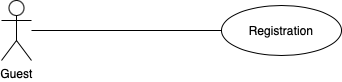
\includegraphics[width=0.6\linewidth]{Images/UCD_Registration.png}
        \caption{Guest Diagram}
        \label{fig:class_diagram}%
    \end{center}
\end{figure}

\subsection{Student}
\begin{figure}[H]
    \begin{center}
        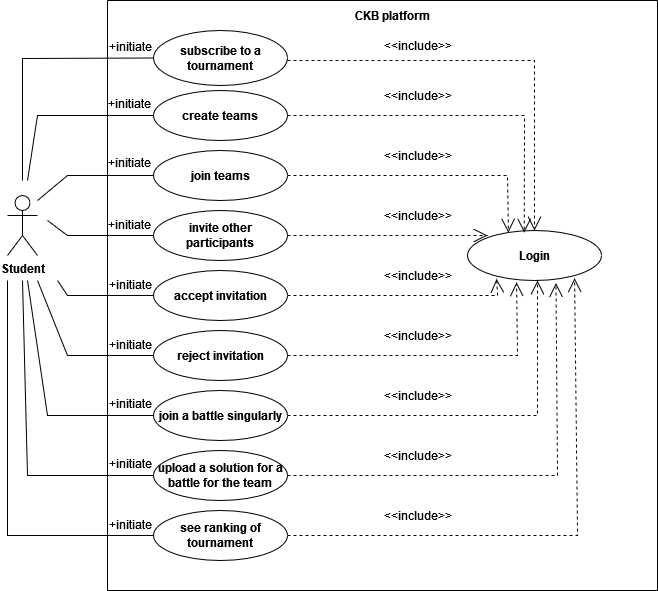
\includegraphics[width=0.8\linewidth]{Images/UCD_Student.png}
        \caption{Student Diagram}
        \label{fig:class_diagram}%
    \end{center}
\end{figure}
\subsection{Educator}
\begin{figure}[H]
    \begin{center}
        \includegraphics[width=0.8\linewidth]{Images/UCD_Educators.png}
        \caption{Educator Diagram}
        \label{fig:class_diagram}%
    \end{center}
\end{figure}

\section{Use Cases}
\label{subsec: use_case}%
\newcounter{uc}
\setcounter{uc}{1}
\newcommand{\cuc}{\theuc\stepcounter{uc}}
In this section, the primary identified use cases are elucidated. 
Each use case is accompanied by a table delineating entry conditions, event flow, exit conditions, and exceptions. 
Additionally, a sequence diagram is provided to illustrate the interactions between entities and the functions invoked. 
This comprehensive representation aims to capture the essential aspects of each use case, ensuring a clear understanding of the system dynamics within the context of the Code Kata Battle (CKB) platform.
\subsubsection*{UC\cuc . Student Registration}
\begin{center}
    \begin{longtable}{lp{0.75\linewidth}}
        \hline
        Actor            & Unregistered Student                                                                                                                                                                               \\
        \hline
        Entry conditions & The student isn't registered on the \verb|CKB| platform and clicks the sign-up button                                                                                                               \\
        \hline
        Event Flow       
        & 1. The \verb|CKB| platform prompts the unregistered student to input personal information (name, surname, email linked to an institutional profile).\\
        & 2. The unregistered student fills the form with personal information\\
        & 3. The student agrees to the platform's "Terms \& Conditions," and "Privacy Policy."\\
        & 4. The \verb|CKB| platform validates the provided student information.\\
        & 5. The \verb|CKB| platform requests the student to input a username for their profile.\\
        & 6. The student inputs a username.\\ 
        & 7. The \verb|CKB| platform validates the username.\\
        & 8. The \verb|CKB| platform sends a verification email containing a 6-digit code to the student's provided institutional email address.\\
        & 9. The \verb|CKB| platform prompts the student to input the verification code.\\
        & 10. The student inputs the verification code.\\
        & 11. The \verb|CKB| platform communicates the outcome of the student's registration.\\
        \hline
        Exit condition   & An account is created.   \\                                                                                                                                                                           
        \hline
        Exceptions   
        & 3.1. The student does not agree to the platform's "Terms \& Conditions," and "Privacy Policy."\\
            & The \verb|CKB| platform shows a message asking the user to agree to such "Terms \& Conditions" stopping the sign up operation.  \\                                                                                                   
        & 4.1. The \verb|CKB| platform is unable to validate the student's personal information.  \\                                                                                                         
            & In these cases, the unregistered student receives a notification with an error message.   \\
        & 7.1. The student's provided username is already in use.           \\                                                                                                
            & The \verb|CKB| platform shows a message asking the user to choose another username.   \\
        & 7.2. The student's provided username is in a non acceptable format    \\
            & The \verb|CKB| platform shows a message asking the user to choos another username    \\
      % email not received by user                                                                                        \\
        & 10.1. The student inputs an incorrect verification code.      \\                                                           
            & The \verb|CKB| platform shows a message asking the user to input the correct verification code.  \\
                                                                                        
        \hline
        \caption{Student Registration Use Case.}
        \label{tab: student_registration_use_case}
    \end{longtable}

    %QUI SEQUENCE DIAGRAM
    %\begin{comment}
    %    \begin{figure} [H]
    %        \begin{center}
                %\includegraphics[width=0.9\linewidth]{Images/SequenceDiagrams/student_registration}
   %             \caption{Student Registration Sequence Diagram}
%                \label{fig: student_registration_seq_diag}
    %        \end{center}
   %     \end{figure}
    %    \end{comment}
\end{center}

\subsubsection*{UC\cuc . User Login}
\begin{center}
    \begin{longtable}{lp{0.75\linewidth}}
        \hline
        Actor            & Registered User                                                                                                                                                                               \\
        \hline
        Entry conditions & The User is registered on the \verb|CKB| platform and clicks the login button.                                                                                                               \\
        \hline
        Event Flow       
        & 1. The \verb|CKB| platform prompts the user to input institutional email.\\
        & 2. The \verb|CKB| platform validates the email redirecting the user to the institution's page.\\
        & 3. The \verb|CKB| platform communicates the outcome of the user's login.\\
        \hline
        Exit condition   & Login completed.   \\                                                                                                                                                                           
        \hline
        Exceptions   
        & 2.1. The user's email isn't valid.\\                                          
        & 2.2. The user's verification on the institution's page goes wrong. \\                                                                                                         
            & In these cases, the user receives a notification with an error message.   \\                                                               
        \hline
        \caption{User Login Use Case.}
        \label{tab: user_login_use_case}
    \end{longtable}

    %QUI SEQUENCE DIAGRAM
    %\begin{comment}
    %    \begin{figure} [H]
    %        \begin{center}
                %\includegraphics[width=0.9\linewidth]{Images/SequenceDiagrams/student_registration}
   %             \caption{Student Registration Sequence Diagram}
%                \label{fig: student_registration_seq_diag}
    %        \end{center}
   %     \end{figure}
    %    \end{comment}
\end{center}

\subsubsection*{UC\cuc . Student Subscription to a Tournament}
\begin{center}
    \begin{longtable}{lp{0.75\linewidth}}
        \hline
        Actor            & Registered Student                                                                                                                                                                               \\
        \hline
        Entry conditions & The Student is logged in on the \verb|CKB| platform and clicks to the subscription button to a tournament.                                                                                                            \\
        \hline
        Event Flow       
        & 1. The \verb|CKB| platform receives the request.\\
        & 2. The \verb|CKB| platform checks if the tournament's subscription deadline is over.\\
        & 3. The \verb|CKB| platform communicates the outcome of the student's subscription.\\
        \hline
        Exit condition   & Subscription completed.   \\                                                                                                                                                                           
        \hline
        Exceptions   
        & 2.1. The tournament's subscription deadline is over.\\                                                                                                                                              
            & In these cases, the student receives a notification with an error message.   \\                                                               
        \hline
        \caption{Student Subscription Use Case.}
        \label{tab: student_subscription_use_case}
    \end{longtable}

    %QUI SEQUENCE DIAGRAM
    %\begin{comment}
    %    \begin{figure} [H]
    %        \begin{center}
                %\includegraphics[width=0.9\linewidth]{Images/SequenceDiagrams/student_registration}
   %             \caption{Student Registration Sequence Diagram}
%                \label{fig: student_registration_seq_diag}
    %        \end{center}
   %     \end{figure}
    %    \end{comment}
\end{center}
\subsubsection*{UC\cuc . Educator creates a tournament}

\begin{center}
    \begin{longtable}{lp{0.75\linewidth}}
        \hline
        Actor            & Educator                                                                                                                                                                               \\
        \hline
        Entry conditions & The educator is logged in on the \verb|CKB| platform.\\                                                                                                               \\
        \hline
        Event Flow       
        & 1. The educator clicks on the "Create Tournament" button from the Menu in the homepage.\\
        & 2. The \verb|CKB| platform prompts the educator to input the tournament name.\\
        & 3. The educator inputs the tournament name.\\
        & 4. The \verb|CKB| platform prompts the educator to input the registration deadline.\\
        & 5. The educator inputs the registration deadline.\\
        & 6. The educator toggles the "Advanced Options" section.\\
        & 7. The \verb|CKB| platform prompts the educator to choose whether to include badges or not.\\
        & 8. The educator chooses whether to include badges or not.\\
        & 9. The \verb|CKB| platform prompts the educator to choose which badges to include.\\
        & 10. The educator chooses which badges to include.\\
        & 11. The \verb|CKB| platform prompts the educator to choose whether to create new badges or not.\\
        & 12. The educator chooses to create new badges.\\
        & 13. The \verb|CKB| platform opens a pop-up window allowing the educator to create new badges by selecting and combining variables and rules.\\
        & 14. The educator creates new badges.\\
        & 15. The educator pushes the "Create Tournament" button.\\
        & 16. The \verb|CKB| platform communicates the outcome of the tournament creation.\\
        & 17. The \verb|CKB| platform notifies all students that a new tournament is available.\\
        \hline
        Exit condition   & A tournament is created.   \\                                                                                                                                                                         
        \hline
        Exceptions   
        & 3.1. The educator does not input the tournament name.\\
            & The \verb|CKB| platform shows a message asking the user to input the tournament name.  \\
        & 5.1. The educator does not input the registration deadline or inputs an invalid date.\\
            & The \verb|CKB| platform shows a message asking the user to input the registration deadline.  \\
        & 8.1. The educator does not choose whether to include badges or not.\\
            & The \verb|CKB| platform assumes that badges are not included.  \\
        & 10.1. The educator does not choose which badges to include.\\
            & The \verb|CKB| platform assumes that no pre-existing badges are included.  \\
        & 12.1. The educator does not choose to create new badges.\\
            & The \verb|CKB| platform assumes that no new badges are created.  \\
        & 14.1. The educator tries to create a new badge without selecting any variable or rule.\\
            & The \verb|CKB| platform shows a message asking the user to select at least one variable or rule.  \\
        \hline
        \caption{Tournament Creation Use Case.}
        \label{tab: tournament_creation_use_case}
    \end{longtable}

    %QUI SEQUENCE DIAGRAM
    %\begin{comment}
    %    \begin{figure} [H]
    %        \begin{center}
                %\includegraphics[width=0.9\linewidth]{Images/SequenceDiagrams/tournament_creation}
   %             \caption{Tournament Creation Sequence Diagram}
%                \label{fig: tournament creation_seq_diag}
    %        \end{center}
   %     \end{figure}
    %    \end{comment}
\end{center}


\subsubsection*{UC\cuc . Educator closes a tournament}
\begin{center}
    \begin{longtable}{lp{0.75\linewidth}}
        \hline
        Actor            & Educator \\
        \hline
        Entry conditions & The educator is logged in on the \verb|CKB| platform and has permissions to perform actions on a specific tournament.\\                                                                                                               \\
        \hline
        Event Flow       
        & 1. The educator clicks on a tournament for which he has editing permissions from the list in the "Tournaments" page\\
        & 2. The \verb|CKB| platform shows the tournament details page\\
        & 3. The educator clicks on the "Close Tournament" button\\
        & 4. The \verb|CKB| platform shows a pop-up window asking for confirmation\\
        & 5. The educator confirms the action\\
        & 6. The \verb|CKB| platform communicates the outcome of the tournament closing\\
        & 7. The \verb|CKB| computes the final ranking of the tournament and makes it available\\
        & 8. The \verb|CKB| platform notifies all students that the tournament is closed\\
        \hline
        Exit condition   & The tournament is closed.   \\                                                                                                                                                                         
        \hline
        Exceptions   
        & 5.1. The educator does not confirm the action\\
            & The \verb|CKB| platform does not close the tournament.  \\
        \hline
        \caption{Tournament Closing Use Case.}
        \label{tab: tournament_closing_use_case}
    \end{longtable}

    %QUI SEQUENCE DIAGRAM
    %\begin{comment}
    %    \begin{figure} [H]
    %        \begin{center}
                %\includegraphics[width=0.9\linewidth]{Images/SequenceDiagrams/tournament_closing}
   %             \caption{Tournament Closing Sequence Diagram}
%                \label{fig: tournament_closing_seq_diag}
    %        \end{center}
   %     \end{figure}
    %    \end{comment}
\end{center}

%. To create a new battle, an educator uses the CKB
%platform to perform the following steps:
%• upload the code kata (description and software project, including test cases and build
%automation scripts),
%• set minimum and maximum number of students per group,
%• set a registration deadline,
%• set a final submission deadline,
%• set additional configurations for scoring (see further details in the following).


\subsubsection*{UC\cuc . Educator creates a new Code Kata Battle}
\begin{center}
    \begin{longtable}{lp{0.75\linewidth}}
        \hline
        Actor            & Educator \\
        \hline
        Entry conditions & The educator is logged in on the \verb|CKB| platform and is on a tournament's details page. The educator has permissions to add new CKB to the tournament.\\                                                                                                               \\
        \hline
        Event Flow      
        & 1. The educator clicks on the "Create New Code Kata Battle" button\\ 
        & 2. The \verb|CKB| platform asks the educator to upload the code kata for the battle\\
        & 3. The educator uploads the code kata\\
        & 4. The \verb|CKB| platform verifies that the code kata includes a description and a software project with test cases and build automation scripts\\
        & 5. The \verb|CKB| platform asks the educator to set the minimum and maximum number of students per group\\
        & 6. The educator sets the minimum and maximum number of students per group\\
        & 7. The \verb|CKB| platform asks the educator to set a registration deadline\\
        & 8. The educator sets a registration deadline\\
        & 9. The \verb|CKB| platform asks the educator to set a final submission deadline\\
        & 10. The educator sets a final submission deadline\\
        & 11. The educator clicks on the "Additional Configurations for Scoring" button\\
        & 12. The \verb|CKB| platform shows the "Additional Configurations for Scoring" section\\
        & 13. The educator sets additional configurations for scoring if needed\\
        & 14. The educator clicks on the "Create" button\\
        & 15. The \verb|CKB| platform communicates the outcome of the CKB creation\\
        & 16. The \verb|CKB| platform notifies all students subscribed to the tournament that a new CKB is available\\
        \hline
        Exit condition   & The new CKB is added to the tournament.   \\                                                                                                                                                                         
        \hline
        Exceptions   
        & 4.1. The code kata does not include a description\\
            & The \verb|CKB| platform shows a message asking the educator to upload a code kata including a description.  \\
        & 4.2. The code kata does not include a software project\\
            & The \verb|CKB| platform shows a message asking the educator to upload a code kata including a software project.  \\
        & 4.3. The code kata does not include test cases\\
            & The \verb|CKB| platform shows a message asking the educator to upload a code kata including test cases.  \\
        & 4.4. The code kata does not include build automation scripts\\
            & The \verb|CKB| platform shows a message asking the educator to upload a code kata including build automation scripts.  \\
        & 5.1. The educator does not set the minimum and maximum number of students per group\\
            & The \verb|CKB| platform shows a message asking the educator to set the minimum and maximum number of students per group.  \\
        & 7.1. The educator does not set a registration deadline or sets an invalid date\\
            & The \verb|CKB| platform shows a message asking the educator to set a registration deadline.  \\
        & 9.1. The educator does not set a final submission deadline or sets an invalid date\\
            & The \verb|CKB| platform shows a message asking the educator to set a final submission deadline.  \\
        \hline
        \caption{New CKB creation Use Case.}
        \label{tab: new_CKB_use_case}
    \end{longtable}

    %QUI SEQUENCE DIAGRAM
    %\begin{comment}
    %    \begin{figure} [H]
    %        \begin{center}
                %\includegraphics[width=0.9\linewidth]{Images/SequenceDiagrams/CKB_creation}
   %             \caption{CKB creation Sequence Diagram}
%                \label{fig: ckb_creation_seq_diag}
    %        \end{center}
   %     \end{figure}
    %    \end{comment}
\end{center}


% Tournaments are created by an educator. Each battle created by an educator belongs to a specific tournament. Tournaments are created by an
%educator who can then grant to other colleagues the permission to create battles within the context of a specific tournament

\subsubsection*{UC\cuc . Educator grants another educator permissions to create battles in a tournament}
\begin{center}
    \begin{longtable}{lp{0.75\linewidth}}
        \hline
        Actor            & Educator \\
        \hline
        Entry conditions & The educator is logged in on the \verb|CKB| platform and is on a tournament's details page. The educator is the creator of the tournament.\\
        \hline
        Event Flow      
        & 1. The educator clicks on the "Add Administrator" button\\
        & 2. The \verb|CKB| platform asks the educator to input the email or username of the educator to whom grant permissions\\
        & 3. The educator inputs the email or username of the educator to whom grant permissions\\
        & 4. The \verb|CKB| platform communicates the outcome of the operation\\
        & 5. The \verb|CKB| platform notifies the educator to whom permissions have been granted\\
        \hline
        Exit condition   & The educator to whom permissions have been granted can create battles in the tournament.   \\
        \hline
        Exceptions   
        & 3.1. The educator inputs an invalid email or username or one belonging to a user who is not an educator\\
            & The \verb|CKB| platform shows a message asking the educator to input a valid email or username.  \\
        \hline
        \caption{New CKB creation Use Case.}
        \label{tab: grant_permissions_use_case}
    \end{longtable}

    %QUI SEQUENCE DIAGRAM
    %\begin{comment}
    %    \begin{figure} [H]
    %        \begin{center}
                %\includegraphics[width=0.9\linewidth]{Images/SequenceDiagrams/grant_premissions}
   %             \caption{Granting another Educator permissions to create new CKB Sequence Diagram}
%                \label{fig: granting_permissions_seq_diag}
    %        \end{center}
   %     \end{figure}
    %    \end{comment}
\end{center}


%The CKB platform also includes gamification badges: elements in the form of rewards that represent
%the achievements of individual students. Badges are defined by educators when they create a
%tournament. Each badge has a title (e.g., “top committer”) and one or more rules (i.e., simple Boolean properties) that must be fulfilled to achieve the badge. 
%Thus, each badge is assigned to one or more students depending on the rules checked at the end of the tournament. 
%The following are examples of possible badges:
%    • Title: tournament participant
%        o Rules: { tot_attended_battles > 0 }
%    • Title: top committer
%        o Rules: { tot_commits_student == max_tot_commits }
%Where tot_attended_battles, tot_commits_student and max_tot_commits are pre-defined variables
%that represent, respectively, the total number of battles the student has been involved in, the number
%of commits carried out by the student and the maximum total number of commits considering all
%students.
%As mentioned above, educators can create new badges and define new rules as well as new variables
%associated with them. Variables can represent any piece of information available in CKB relevant for
%scoring. It is up to you to identify such information and a simple language for creating new variables,
%rules, and badges.
        

\subsubsection*{UC\cuc . Educator creates a new badge}
\begin{center}
    \begin{longtable}{lp{0.75\linewidth}}
        \hline
        Actor            & Educator \\
        \hline
        Entry conditions & The educator is logged in on the \verb|CKB| platform and is on a tournament's details page. The educator is creating a tournament.\\
        \hline
        Event Flow      
        & 1. The educator clicks on the "Create New Badge" button in "Advanced Options"\\
        & 2. The \verb|CKB| platform prompts the educator to input the title of the badge\\
        & 3. The educator inputs the title of the badge\\
        & 4. The \verb|CKB| platform allows the educator to create new variables and rules for the badge\\
        & 5. The educator defines the rules of the badge through a wizard\\
        & 6. The educator clicks on the "Create" button\\
        & 7. The \verb|CKB| platform communicates the outcome of the badge creation\\
        \hline
        Exit condition   & The new badge is added to the tournament.   \\
        \hline
        Exceptions
        & 3.1. The educator does not input the title of the badge\\
            & The \verb|CKB| platform shows a message asking the educator to input the title of the badge.  \\
        & 5.1. The educator does not define any rule for the badge\\
            & The \verb|CKB| platform shows a message asking the educator to define at least one rule for the badge.  \\
        \hline
        \caption{New Badge creation Use Case.}
        \label{tab: badge_creation_use_case}
    \end{longtable}

    %QUI SEQUENCE DIAGRAM
    %\begin{comment}
    %    \begin{figure} [H]
    %        \begin{center}
                %\includegraphics[width=0.9\linewidth]{Images/SequenceDiagrams/badge_creation}
   %             \caption{New Badge creation Sequence Diagram}
%                \label{fig: new_badge_creation_seq_diag}
    %        \end{center}
   %     \end{figure}
    %    \end{comment}
\end{center}

\section{Performance Requirements}
\label{subsec:performance_requirements}%

\subsection*{1. Response Time:}
   - The \verb|CKB| platform shall respond to user interactions within an average time of 2 seconds, measured from the user action initiation to the completion of the corresponding operation.

\subsection*{2. Concurrent Users:}
   - The platform should support at least 1000 concurrent users without a significant degradation in response time.

\subsection*{3. GitHub Integration:}
   - GitHub repository creation and updates triggered by student commits shall be processed within 5 minutes of the GitHub action.

\subsection*{4. Automated Evaluation:}
   - Automated evaluation of submitted code shall be completed within 1 minute of each GitHub push action.

\subsection*{5. Scalability:}
   - The platform should accommodate at least a 20\% annual increase in user base and battle participation.

\subsection*{6. Data Retrieval Time:}
   - Information retrieval for ongoing tournaments, tournament ranks, and personal scores should be performed within an average time of 3 seconds.

\subsection*{7. Consolidation Stage:}
   - The consolidation stage, where manual evaluation is required, should be completed within 3 days after the submission deadline of a battle.

\subsection*{8. Badge Assignment:}
   - Badge assignment based on rules and variables should be executed within 1 day after the final tournament rank becomes available.

\subsection*{9. Platform Uptime:}
   - The platform should maintain a minimum of 99.9\% uptime over any given month.

\subsection*{10. Notification Latency:}
    - Notifications should be sent to all relevant users within 1 minute of the triggering event.

\subsection*{11. Gamification Features:}
    - Display of badges on user profiles and visualization of tournament-related achievements should be accessible within a response time of 3 seconds.

\subsection*{12. API Response Time:}
    - External APIs used for integrations should respond within 5 seconds.

\subsection*{13. Load Testing:}
    - The platform should undergo periodic load testing to handle peak loads without compromising performance.

\subsection*{14. Security Scan Duration:}
    - Security scans during code quality evaluation should not exceed 2 minutes.







\begin{comment}
\section{Performance Requirements}
\label{subsec:performance_requirements}%

\subsection*{1. Response Time:}
   - The CKB platform shall respond to user interactions (e.g., creating a battle, joining a battle, submitting code) within an average time of 2 seconds, measured from the user action initiation to the completion of the corresponding operation.

\subsection*{2. Concurrent Users:}
   - The platform should support at least 1000 concurrent users participating in different battles and tournaments without a significant degradation in response time.

\subsection*{3. GitHub Integration:}
   - GitHub repository creation and updates triggered by student commits shall be processed and reflected in the CKB platform within 5 minutes of the GitHub action.

\subsection*{4. Automated Evaluation:}
   - The automated evaluation of submitted code, including functional aspects, timeliness, and quality level, shall be completed within 1 minute of each GitHub push action.

\subsection*{5. Scalability:}
   - The CKB platform should be designed to handle a growth in the number of users, battles, and tournaments. It should accommodate at least a 20\% annual increase in user base and battle participation.

\subsection*{6. Data Retrieval Time:}
   - Information retrieval for ongoing tournaments, tournament ranks, and personal scores should be performed within an average time of 3 seconds.

\subsection*{7. Consolidation Stage:}
   - The consolidation stage, where manual evaluation is required, should be completed within 3 days after the submission deadline of a battle.

\subsection*{8. Badge Assignment:}
   - Badge assignment based on rules and variables should be executed within 1 day after the final tournament rank becomes available.

\subsection*{9. Platform Uptime:}
   - The CKB platform should maintain a minimum of 99.9\% uptime over any given month to ensure continuous availability for users.

\subsection*{10. Notification Latency:}
    - Notifications, such as battle creation, submission deadlines, and tournament closure, should be sent to all relevant users within 1 minute of the triggering event.

\subsection*{11. Gamification Features:}
    - The display of badges on user profiles and the visualization of tournament-related achievements should be accessible with a response time of 3 seconds.

\subsection*{12. API Response Time:}
    - Any external APIs used for integrations, such as GitHub Actions and static analysis tools, should respond within 5 seconds to avoid delays in platform functionalities.

\subsection*{13. Load Testing:}
    - The platform should undergo periodic load testing to ensure it can handle peak loads and unexpected spikes in user activity without compromising performance.

\subsection*{14. Security Scan Duration:}
    - The time required for security scans during the evaluation of code quality should not exceed 2 minutes.

\end{comment}


\section{Design Constraints}
\label{sec:design_constraints}%

\subsection{Standards Compliance}
\label{subsec:standards_compliance}%
The Code Kata Battle (CKB) platform must conform to established standards and legal requirements to ensure ethical and lawful operation. Key considerations include:

\begin{enumerate}
    \item \textbf{Privacy and Data Laws:}
          \begin{itemize}
              \item The platform must adhere to all laws governing privacy and data treatment, especially regarding user information and data exchange with third parties, such as CodeKata educators.
              \item Compliance with the European Union General Data Protection Regulation (EU GDPR) is mandatory to ensure the privacy and rights of users are protected.
          \end{itemize}

    \item \textbf{EU GDPR Principles:}
          \begin{itemize}
              \item The system design should align with the principles outlined in Article 5 of the GDPR document, emphasizing the lawful, fair, and transparent processing of personal data.
          \end{itemize}
\end{enumerate}

\subsection{Hardware Limitations}
\label{subsec:hardware_limitations}%
The design and functionality of the CKB platform need to consider specific limitations for optimal user experience:

\begin{enumerate}
    \item \textbf{Cross-Platform Accessibility:}
          \begin{itemize}
              \item The platform should be accessible from both web browsers and mobile applications. Mobile applications will be implemented for Android and iOS operating systems.
          \end{itemize}
\end{enumerate}
\textbf{Note:} Cross-platform accessibility, although listed under hardware limitations, primarily involves software compatibility rather than hardware constraints. It highlights the need for the platform to function seamlessly across different operating systems.

\subsection{Other Constraints}
While considering standard compliance and hardware limitations, additional constraints specific to the CKB project should be acknowledged:

\begin{enumerate}
    \item \textbf{Educator Configuration:}
          \begin{itemize}
              \item The design should facilitate easy configuration by educators, allowing them to customize scoring criteria, badge rules, and associated variables according to their preferences and requirements.
          \end{itemize}

    \item \textbf{Automated Testing Tools:}
          \begin{itemize}
              \item Seamless integration with automated testing tools is essential. The platform should be designed to accommodate any constraints or limitations imposed by these tools during code evaluation.
          \end{itemize}

    \item \textbf{Scalability:}
          \begin{itemize}
              \item The platform must be scalable to handle a growing user base, increasing numbers of battles, and additional features without compromising performance. Consideration should be given to both the user interface and backend infrastructure.
          \end{itemize}

    \item \textbf{Educator Workload:}
          \begin{itemize}
              \item The design should optimize the educator's workload, particularly during the manual evaluation stage. Streamlining the evaluation process will enhance efficiency and user satisfaction.
          \end{itemize}

    \item \textbf{Gamification Logic:}
          \begin{itemize}
              \item Constraints associated with the gamification logic, including badge creation, rule definition, and variable association, should be carefully considered to maintain system flexibility without compromising integrity.
          \end{itemize}

    \item \textbf{Integration with External Systems:}
          \begin{itemize}
              \item The platform needs to seamlessly integrate with external systems, such as GitHub, while considering any constraints or limitations imposed by these external systems on data exchange and interactions.
          \end{itemize}
\end{enumerate}

These design constraints are vital to guide the development of the Code Kata Battle platform, ensuring legal compliance, optimal user experience, and consideration of specific project-related constraints.




\section{Software System Attributes}
\label{sec:software_system_attributes}%

\subsection{Reliability}
\label{subsec:reliability}%
The reliability of the Code Kata Battle (CKB) platform is crucial for its users, especially during critical operations such as code evaluations and scoring. 
While the platform doesn't require absolute perfection in every operation, it must maintain a high level of reliability to instill confidence in educators and students. 
Considering the nature of the platform, a failure rate between $0.1\%$ and $1\%$ is deemed acceptable. 
This range positions the CKB system as a robust and dependable tool for code kata battles.

\subsection{Availability}
\label{subsec:availability}%
Availability is a key attribute for the CKB platform, particularly for educators who rely on its functionalities for managing tournaments, battles, and student assessments. 
Downtime, especially during crucial periods like ongoing battles or tournament deadlines, is unacceptable. Therefore, the platform aims to achieve a remarkable $99.9\%$ uptime, ensuring educators have uninterrupted access to critical features. 
This commitment to high availability enhances the overall user experience and reinforces the platform's reliability.

\subsection{Security}
\label{subsec:security}%
Security is paramount for the CKB platform, given its involvement in handling code submissions, communication with external systems like GitHub, and the storage of sensitive user information. 
The platform ensures data privacy by employing HTTPS for secure communication. Additionally, all stored information is encrypted, providing an extra layer of protection against potential security threats. 
By prioritizing these security measures, the CKB platform safeguards the integrity and confidentiality of user data, fostering trust among educators and students.

\subsection{Maintainability}
\label{subsec:maintainability}%
Maintainability is a critical aspect of the CKB platform's design philosophy. The platform is structured into modular components to facilitate efficient maintenance, updates, and future extensions. 
Each implemented functionality is meticulously documented, ensuring clarity for developers involved in maintenance tasks. 
The design emphasizes a modular approach, allowing updates to specific components without adversely affecting the entire system. 
This commitment to maintainability ensures that the CKB platform can adapt to evolving requirements and technologies without compromising its stability.

\subsection{Portability}
\label{subsec:portability}%
The CKB platform prioritizes portability to accommodate a diverse user base. Users can access the platform seamlessly from web browsers and mobile applications on both Android and iOS devices. 
The choice of programming languages and development tools is a strategic decision, with the goal of providing a consistent user experience across different platforms. 
While cross-platform development tools offer efficiency, separate implementations for Android and iOS are considered for a more tailored user experience. 
This flexibility in portability ensures that the CKB platform remains accessible and user-friendly, regardless of the chosen device or operating system.



    \chapter{Formal Analysis Using Alloy}
    \label{ch:formal_analysis_using_alloy}%
    Hey


    \chapter{Effort Spent}
    \label{ch:effort_spent}%
    \begin{table}[H]
    \begin{center}
        \begin{tabular}{c|c}
            \hline
            Member of group & Effort spent \\
            \hline
            Federico Zanca & \begin{tabular}{p{0.25\linewidth}|c}
                             Introduction          & $0h$  \\
                             Overall description   & $0h$ \\
                             Specific requirements & $0h$ \\
                             Formal analysis       & $0h$ \\
                             Reasoning             & $0h$ \\
            \end{tabular} \\
            \hline
            Federico Costantini & \begin{tabular}{p{0.25\linewidth}|c}
                             Introduction          & $0h$  \\
                             Overall description   & $0h$ \\
                             Specific requirements & $0h$ \\
                             Formal analysis       & $0$  \\
                             Reasoning             & $0h$ \\
            \end{tabular} \\
            \hline
            Michele Zhenghao Zhuge & \begin{tabular}{p{0.25\linewidth}|c}
                                     Introduction          & $0h$ \\
                                     Overall description   & $0h$ \\
                                     Specific requirements & $0h$ \\
                                     Formal analysis       & $0h$ \\
                                     Reasoning             & $0h$ \\
            \end{tabular} \\
            \hline
        \end{tabular}
        \caption{Effort spent by each member of the group.}
        \label{tab:effor_spent}
    \end{center}
\end{table}



    \chapter{References}
    \label{ch:references}%
    \section{Paper and online references}
\label{sec:paper_references}%
\begin{itemize}
    \item \href{https://polimi365-my.sharepoint.com/:b:/g/personal/10710351_polimi_it/EZXUPFfeFKdBkf5M8W-EBYgB2JrrVLr23BYJ4MXQ7kzUkA?e=o0wvyw}{The specification document Assignment RDD AY 2023-2024.pdf}
    \item \href{https://www.codewars.com/}{An example of a website with similar features to the CKB platform}
\end{itemize}


\section{Used tools}
\label{sec:used_tools}%
\begin{itemize}
    \item \href{https://github.com/}{GitHub} for project versioning
    \item \href{https://draw.io/}{Draw.io} for UML diagrams
    \item \href{https://www.notion.so/}{Notion} for reasoning, notes and task assignment between members of the group
    \item \href{https://code.visualstudio.com/}{Visutal Studio Code} as \LaTeX\ and Alloy editor
    \item \href{https://alloytools.org/}{Alloy} for formal analysis
\end{itemize}


% LIST OF FIGURES
    \listoffigures

% LIST OF TABLES
    \listoftables
    \cleardoublepage
    \newpage
\end{document}